\section{Diagnosis: Signal Structure in Agent OPD}
\label{sec:diag}

Long-horizon agent OPD still optimizes a teacher-matching loss over a generated
sequence, but the sequence is also an interaction trace.
This section gives a turn-resolved diagnosis of \textbf{how OPD supervision behaves in
long-horizon agent tasks}, focusing on where the teacher signal appears, how
reliably it separates outcomes, and how much loss budget it receives.

% A turn-resolved diagnosis must therefore separate
% three quantities that a flat sequence view conflates: the local teacher-correction
% signal under the student's on-policy contexts, the cost of collecting additional
% turns, and the loss mass assigned to each collected turn. 

\subsection{Raw Turn-Level KL Exposes Non-Uniform Supervision}
\label{sec:diag:surv}

Prior OPD and agent-distillation work has emphasized
long-trajectory exposure and the need for temporal or step-wise treatment
\citep{wang2026tcod,zhong2026sod}. Our diagnosis asks a
complementary question: \textit{How is the reverse-KL supervision itself distributed across turns?}
We begin with the least processed measurement: the mean reverse-KL signal at each model turn during vanilla OPD.

\textbf{Setup.}
We use ALFWorld~\citep{shridhar2021alfworld} and Multi-Hop Search as example tasks.
Both diagnostics use vanilla OPD over 100 optimizer steps: ALFWorld with a Qwen3-4B~\citep{yang2025qwen3} student distilled from a Qwen3-8B-GRPO teacher (ALFWorld-4B), and Multi-Hop Search with a Qwen3.5-2B~\citep{yang2025qwen3} student from a Qwen3.5-9B-GRPO teacher (Multi-Hop Search-2B).
Turn-level means are computed only over trajectories that reach each turn. We plot the longest prefix where each turn is supported by at least 8 surviving trajectories, covers at least 10\% of turn-0 cases, and meets these criteria in at least 60\% of training steps. This flexible rule allows deeper analysis than a strict cutoff while avoiding noisy tails.
Dataset, environment, and teacher model details are in Appendix~\ref{app:envs}.

\begin{figure}[tbp]
\centering
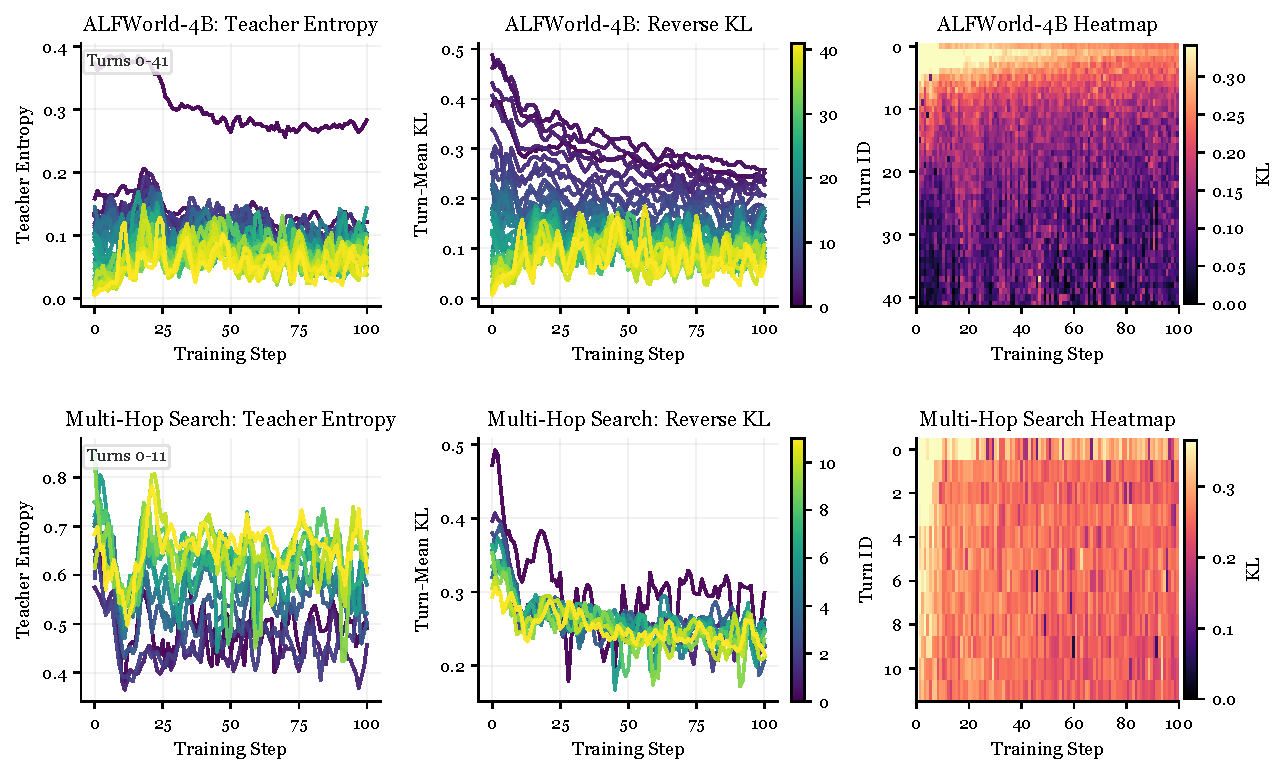
\includegraphics[width=0.95\linewidth]{figures/fig_vanilla_opd_per_turn_kl_alfworld4b_multihop_diagnosis.pdf}
\caption{Turn-resolved teacher uncertainty and reverse-KL under vanilla OPD.
The ALFWorld row uses the Qwen3-4B student baseline, and the Multi-Hop Search
row uses the Qwen3.5-2B student baseline. For each task, the left panel shows
smoothed per-turn teacher entropy, the middle panel shows smoothed per-turn
reverse-KL, and the right panel shows the raw turn-by-step reverse-KL heatmap.
All three panels use the same survivor-supported reliable turn prefix.}
\label{fig:diag-vanilla-turn-kl}
\vspace{-0.2cm}
\end{figure}

\textbf{Result.}
Figure~\ref{fig:diag-vanilla-turn-kl} plots the mean reverse-KL signal at each model turn.
Two patterns are visible. First, teacher uncertainty is itself turn-dependent
and task-dependent. In ALFWorld, deeper turns often have lower teacher
entropy. Multi-Hop Search shows a different entropy
profile: later turns can have higher teacher entropy, yet the
reverse-KL curves are still front-loaded.
Second, the reverse-KL signal is non-uniform and non-stationary over training.
On ALFWorld, early turns start with much larger KL and then drop quickly
during the first 20--30 optimizer steps, while a long tail of later turns
remains lower and noisier. Multi-Hop Search shows a shorter but still structured
profile: the first few turns have the largest KL, and the rest
settle into a narrower band after the initial alignment period. The immediate
conclusion is that vanilla agent OPD cannot be diagnosed by a single average KL.
However, the per-turn KL trend itself is ambiguous: late-turn decay is consistent both
with genuine alignment and with the teacher signal losing discriminative power.
We next test the latter directly.

% \subsection{Entropy-Normalized Local Correction Demand}
% \label{sec:diag:algebra}

% Raw KL mixes two effects: the amount of local teacher correction and the scale
% of the teacher distribution at that turn. We therefore pair per-turn KL with
% teacher entropy. Let $K_t$ be the mean per-token reverse-KL signal at turn $t$,
% and let $H_t$ be the teacher entropy on the same supervised positions. We define
% the entropy-normalized local correction demand as
% \begin{equation}
% \NKL_t = \frac{K_t}{H_t+\epsilon}.
% \label{eq:diag-nkl}
% \end{equation}
% This ratio measures how much local reverse-KL correction remains after accounting
% for the teacher's own uncertainty at the same on-policy context. It gives a
% turn-comparable scale for the correction signal before we reason about rollout
% depth or loss allocation.

% Figure~\ref{fig:diag-nkl-entropy} plots this decomposition over training, using
% the same survivor-support rule as Figure~\ref{fig:diag-vanilla-turn-kl}. In
% ALFWorld, teacher entropy decreases strongly with depth, so the raw-KL decay in
% Figure~\ref{fig:diag-vanilla-turn-kl} partly reflects a sharper teacher
% distribution on later environment states. After entropy normalization, the
% correction-demand curves are much flatter across the reliable prefix, showing
% that the apparent raw-KL collapse overstates how quickly local teacher
% corrections disappear. Multi-hop search exhibits the complementary pattern:
% teacher entropy rises on later search/read turns, while $\NKL_t$ remains most
% concentrated in the first few query/action turns. Thus $\NKL_t$ provides a
% task-normalized view of where local teacher corrections concentrate along the
% turn axis.

% \begin{figure}[htbp]
% \centering
% \includegraphics[width=\linewidth]{figures/fig_vanilla_opd_per_turn_nkl_entropy.pdf}
% \caption{Entropy-normalized local correction demand under vanilla OPD. For each
% task, the left panel plots $\NKL_t=K_t/(H_t+\epsilon)$ over training and the right
% panel plots the corresponding teacher entropy $H_t$. Curves use the same
% survivor-supported turn prefixes as Figure~\ref{fig:diag-vanilla-turn-kl}; NKL
% values are clipped at 6 for readability.}
% \label{fig:diag-nkl-entropy}
% \end{figure}


\subsection{Outcome Separation Degrades and Inverts at Depth}
In a multi-turn setting, raw KL is not necessarily a reliable proxy for the
remaining student--teacher policy gap. We therefore ask a more outcome-oriented
question: at each turn, can KL distinguish rollouts that eventually succeed from
those that eventually fail, and how does this distinction evolve over turn indices and training phases?
For this purpose, define
\begin{equation}
G_t = K_t^{\mathrm{fail}} - K_t^{\mathrm{succ}},
\end{equation}
where $K_t^{\mathrm{fail}}$ and $K_t^{\mathrm{succ}}$ are the per-turn
reverse-KL means computed separately over failed and successful rollouts.
If raw KL were a clean local mismatch signal, failed rollouts should generally
show larger teacher corrections than successful rollouts at the same turn, leading to positive $G_t$.

\begin{figure}[htbp]
\centering
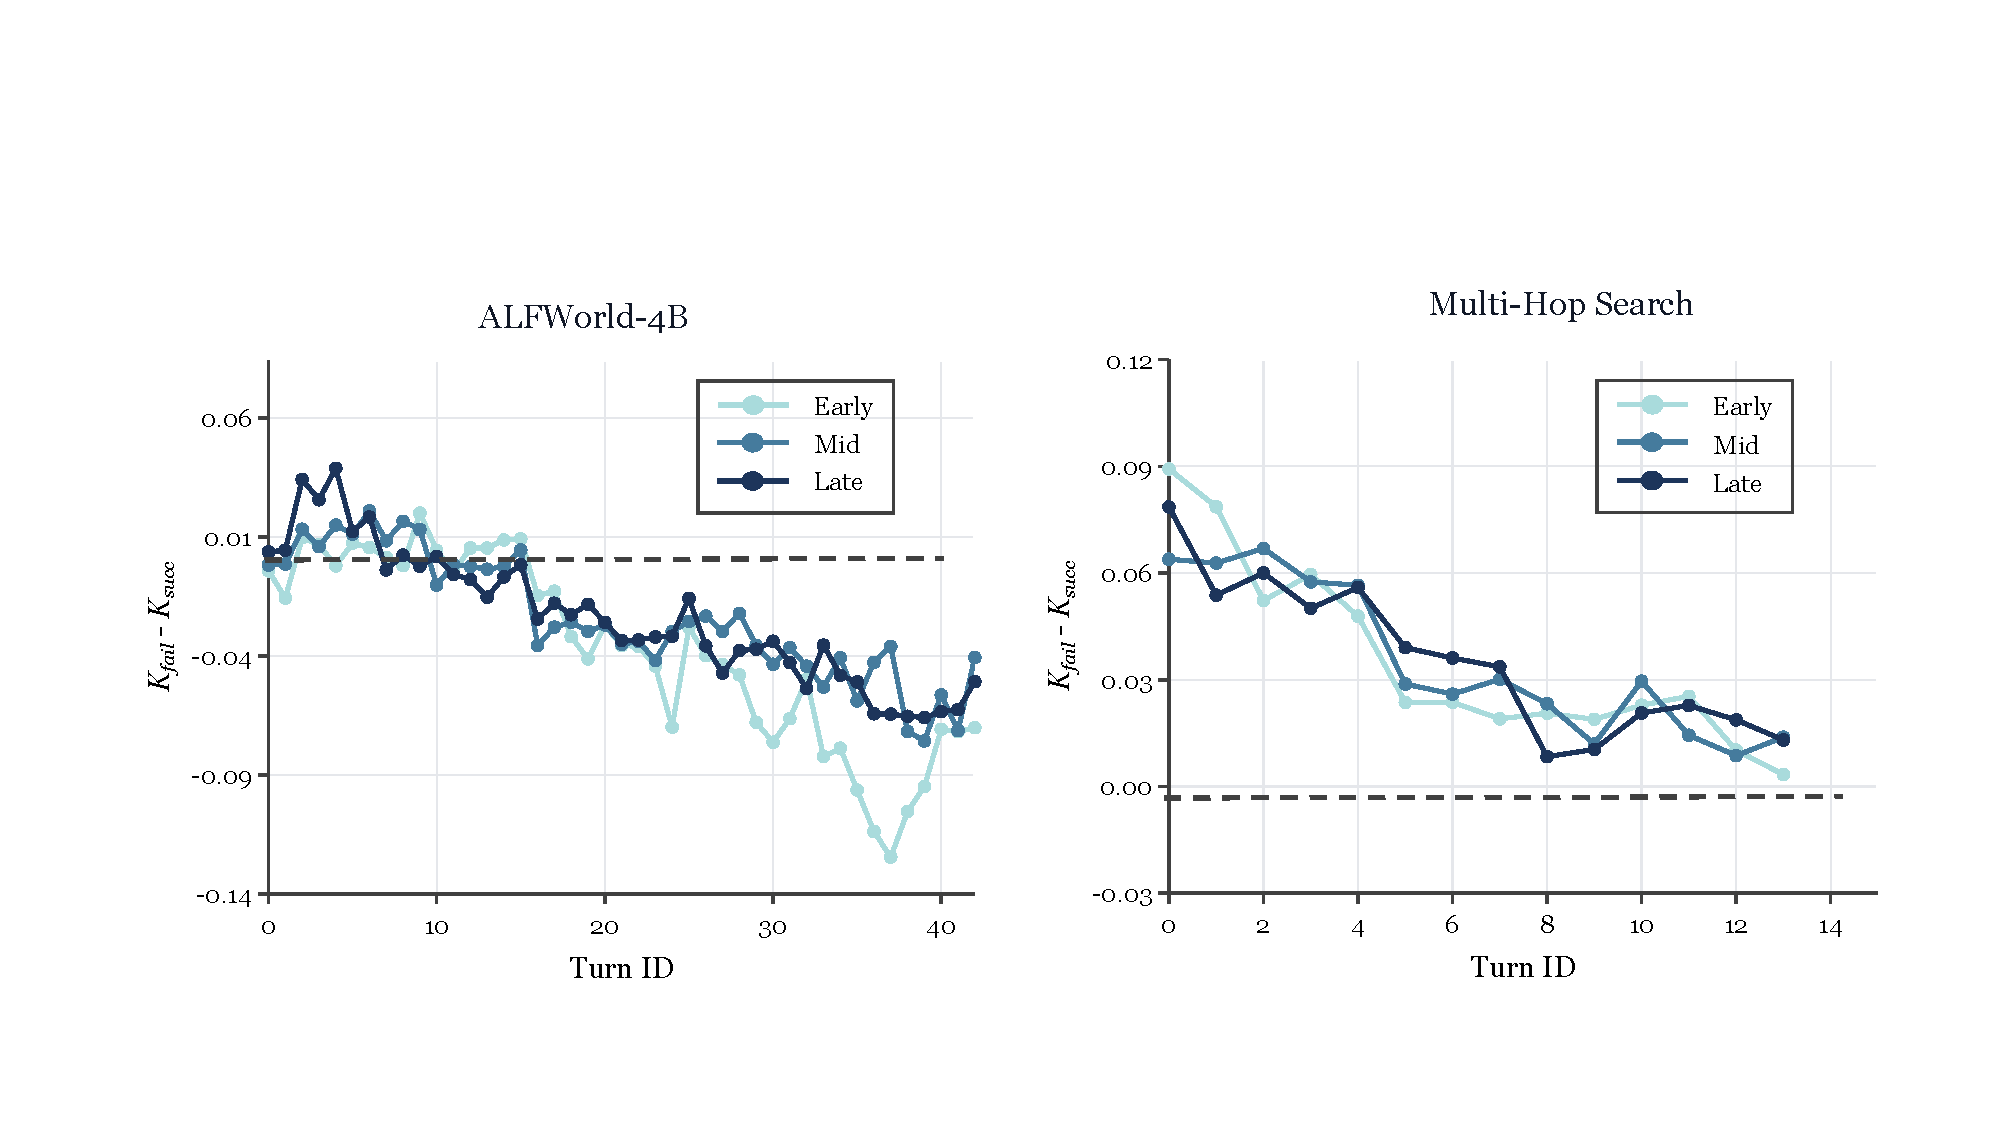
\includegraphics[width=0.85\linewidth]{figures/success_failure_gap.pdf}
\caption{Outcome separation of reverse-KL by turn under vanilla OPD. Each curve
plots the phase mean of $G_t=K_t^{\mathrm{fail}}-K_t^{\mathrm{succ}}$ over early
($0\le$ step $<30$), mid ($30\le$ step $<60$), or late ($60\le$ step $\le100$)
training. Positive values indicate larger KL on failed trajectories.}
\label{fig:diag-success-failure-gap}
\end{figure}

Figure~\ref{fig:diag-success-failure-gap} evaluates whether local KL distinguishes successful from failed trajectories. The sign of $G_t$ varies by task, but both show that deep-turn KL lacks outcome-predictive power.
For ALFWorld, $G_t$ is mostly negative and decreases with depth: successful trajectories often have higher per-turn KL than failed ones, especially at later turns. This is counterintuitive if KL reflects local correction demand, as failed rollouts should need more correction. We attribute this to branch-dependent compression: failed rollouts quickly fall into loops or template-like patterns where both models find the next-token prediction trivial, reducing KL artificially. In contrast, successful rollouts visit more diverse states where the teacher's corrections are less compressed.
In Multi-Hop Search, the gap has the expected positive sign: failed trajectories have larger KL. However, this separation is mostly present in early turns. In later turns, the gap shrinks, demonstrating that KL’s discriminative power is concentrated at the front and weakens with depth.

\subsection{A Contamination-Compression Mechanism}
\label{sec:diag:contamination}

The two measurements above leave a specific ambiguity. Raw reverse-KL decreases
along the reliable turn prefix, and its outcome-separation power also weakens
with depth and can even invert. Therefore a small late-turn KL can have two
different explanations: the student may have learned the teacher, or the
student-generated context may make both models follow the same local
continuation even when their policy-level preferences still differ. We formalize
this ambiguity with a contamination-compression model.

\textbf{Setup.}
Consider a supervised token position in model turn $t$, and let $c$ denote the
full on-policy context before that token, including previous student outputs and
environment/tool observations. Let $\pi_S(\cdot\mid c)$ and
$\pi_T(\cdot\mid c)$ be the next-token distributions of the student and teacher
under the same context. The observable raw KL at turn $t$ is
\begin{equation}
K_t
  = \mathbb{E}_{c\sim\mathcal{C}_t}
  \left[
  \KL\!\left(\pi_S(\cdot\mid c)\,\|\,\pi_T(\cdot\mid c)\right)
  \right],
\label{eq:observed-turn-kl}
\end{equation}
where $\mathcal{C}_t$ is the empirical distribution of supervised token contexts
collected at turn $t$. 
% For the outcome split in
% Figure~\ref{fig:diag-success-failure-gap}, $\mathcal{C}_t^{\mathrm{succ}}$ and
% $\mathcal{C}_t^{\mathrm{fail}}$ denote the corresponding successful and failed
% context distributions, and
% $K_t^{y}=\mathbb{E}_{c\sim\mathcal{C}_t^{y}}[\KL(\pi_S\|\pi_T)]$ for
% $y\in\{\mathrm{succ},\mathrm{fail}\}$. The plotted gap is
% $G_t=K_t^{\mathrm{fail}}-K_t^{\mathrm{succ}}$. These quantities are directly
% measured from the logs. The mechanism below introduces latent quantities only
% to explain why the measured $K_t$ and $G_t$ need not identify the remaining
% policy-level disagreement.

For a fixed context $c$, suppose part of the next-token distribution is nearly
forced by the context itself: repeated strings, formatting constraints, copied
entities, closing delimiters, or low-level continuations that both pretrained
language models assign high probability to. Let $p_F(\cdot\mid c)$ denote this
shared forced component. The remaining mass contains the free component, where
the student and teacher may genuinely disagree. We write
\begin{equation}
\pi_S(\cdot\mid c)
  = \lambda(c) p_F(\cdot\mid c)
    + (1-\lambda(c))p_S^{\mathrm{free}}(\cdot\mid c),
\qquad
\pi_T(\cdot\mid c)
  = \lambda(c) p_F(\cdot\mid c)
    + (1-\lambda(c))p_T^{\mathrm{free}}(\cdot\mid c),
\label{eq:forced-free-mixture}
\end{equation}
where $\lambda(c)\in[0,1]$ is the context-forced mass,
$p_S^{\mathrm{free}}$ is the student's free-component distribution, and
$p_T^{\mathrm{free}}$ is the teacher's free-component distribution. Define the
latent free-component disagreement as
\begin{equation}
\Delta_{\mathrm{free}}(c)
  =
  \KL\!\left(
  p_S^{\mathrm{free}}(\cdot\mid c)
  \,\|\,
  p_T^{\mathrm{free}}(\cdot\mid c)
  \right).
\label{eq:free-component-disagreement}
\end{equation}
Equation~\ref{eq:forced-free-mixture} assumes only that the student and teacher share the context-induced forced component; their free components may differ. In long-horizon settings, increasing student-generated context makes a larger portion of the next-token distribution surface-determined, compressing real decision differences into the remaining free component.

\begin{proposition}[Contamination compression]
\label{prop:contamination-compression}
Under the decomposition in Equation~\ref{eq:forced-free-mixture},
\begin{equation}
\KL\!\left(\pi_S(\cdot\mid c)\,\|\,\pi_T(\cdot\mid c)\right)
\le
(1-\lambda(c))\,
\KL\!\left(
p_S^{\mathrm{free}}(\cdot\mid c)\,\|\,
p_T^{\mathrm{free}}(\cdot\mid c)
\right).
\label{eq:contamination-bound}
\end{equation}
\end{proposition}

% \begin{proof}[Proof sketch]
% Apply the joint convexity of KL to the two mixture components in
% Equation~\ref{eq:forced-free-mixture}, with the shared forced component matched
% to itself. This yields
% \[
% \KL(\lambda p_F+(1-\lambda)p_S^{\mathrm{free}}
% \,\|\,\lambda p_F+(1-\lambda)p_T^{\mathrm{free}})
% \le
% \lambda\KL(p_F\,\|\,p_F)
% +(1-\lambda)\KL(p_S^{\mathrm{free}}\,\|\,p_T^{\mathrm{free}}).
% \]
% The first term is zero, giving Equation~\ref{eq:contamination-bound}. 
% \end{proof}
A full proof is provided in
Appendix~\ref{app:contamination-proof}.


Proposition~\ref{prop:contamination-compression} shows why raw KL is not
identifiable as pure policy disagreement. If
$\Delta_{\mathrm{free}}(c)>0$, the observable fraction of free disagreement
captured by raw KL satisfies
\begin{equation}
\rho(c)
  =
  \frac{
  \KL\!\left(\pi_S(\cdot\mid c)\,\|\,\pi_T(\cdot\mid c)\right)}
  {\Delta_{\mathrm{free}}(c)}
  \le 1-\lambda(c).
\label{eq:compression-ratio}
\end{equation}
Thus a high forced mass $\lambda(c)$ can compress the measured KL even when the
free-component disagreement remains nonzero.

\textbf{Why depth can increase compression.}
In a student rollout, the context at turn $t$ contains all earlier student
outputs and tool observations. Autoregressive generation is positively
self-conditioning: previous high-probability continuations make some future
continuations more predictable, and repeated or format-locked context can
increase the forced mass. It provides a structural explanation for the envelope
seen in Figure~\ref{fig:diag-vanilla-turn-kl}: as the rollout becomes longer,
the measured KL can decay because $(1-\lambda(c_t))$ contracts, not necessarily
because the free-component disagreement has vanished.

\textbf{Asymmetric compression and gap inversion.}
The success/failure gap reveals a stronger version of this mechanism: the
context-forced mass need not be symmetric across outcome branches. Failed
trajectories can exhibit stereotyped patterns, such as repeated invalid
actions, loops over the same subgoal, or template-like continuations. These
patterns are exactly the low-level linguistic regularity and local
self-correlation captured by the forced component $p_F$. Consequently, when the
teacher is conditioned on a failed context, its next-token distribution can be
more strongly locked into the local continuation, making the average forced mass
systematically larger on failed rollouts than on successful ones:
$\lambda_t^{\mathrm{fail}}>\lambda_t^{\mathrm{succ}}$. Successful trajectories,
in contrast, continue to traverse task states and observations; their contexts
remain more information-rich, so the teacher must still make genuine semantic
decisions and the forced mass is lower.

For $y\in\{\mathrm{succ},\mathrm{fail}\}$, let $\bar{\lambda}_t^{y}$ be the
average forced mass and $K_t^{y,\mathrm{free}}$ be the average free-component
reverse-KL among turn-$t$ contexts in outcome group $y$. Reading the compression
bound as a first-order approximation gives
$K_t^{y}\approx(1-\bar{\lambda}_t^{y})K_t^{y,\mathrm{free}}$, and therefore
\begin{equation}
G_t
  \approx
  (1-\bar{\lambda}_t^{\mathrm{fail}})K_t^{\mathrm{fail},\mathrm{free}}
  -
  (1-\bar{\lambda}_t^{\mathrm{succ}})K_t^{\mathrm{succ},\mathrm{free}} .
\label{eq:gap-compression}
\end{equation}
Equation~\ref{eq:gap-compression} explains why the gap can become negative. If
$\bar{\lambda}_t^{\mathrm{fail}}>\bar{\lambda}_t^{\mathrm{succ}}$, the failed
term is suppressed more strongly. Therefore $G_t$ can fall below zero even if
the uncompressed disagreement on failed rollouts is at least as large as that on
successful rollouts. This also explains why the curve can keep decreasing after
it has already become negative. As $t$ grows, failed trajectories accumulate
more degenerate context, so $\bar{\lambda}_t^{\mathrm{fail}}$ can keep
increasing; successful trajectories remain more task-driven, so
$\bar{\lambda}_t^{\mathrm{succ}}$ grows more slowly. The differential
$\bar{\lambda}_t^{\mathrm{fail}}-\bar{\lambda}_t^{\mathrm{succ}}$ therefore
widens with depth, producing the monotone downward trend observed in
Figure~\ref{fig:diag-success-failure-gap}.

% \textbf{Remark B (Asymmetric compression explains gap inversion and monotone descent).}
% Failed trajectories tend to exhibit stereotyped patterns, including repeated
% actions, loops, and template continuations, that are precisely the low-level
% regularities captured by $p_F$. As a result,
% $\lambda(c_t^{S,\mathrm{fail}})$ is systematically higher than
% $\lambda(c_t^{S,\mathrm{succ}})$, so
% Proposition~\ref{prop:contamination-compression} applies more aggressively to
% failed rollouts. This asymmetric compression suppresses
% $K_t^{\mathrm{fail}}$ more than $K_t^{\mathrm{succ}}$, pushing $G_t$ below zero.
% Moreover, because failed trajectories accumulate more degenerate context as
% $t$ grows, the differential
% $\bar{\lambda}_t^{\mathrm{fail}}-\bar{\lambda}_t^{\mathrm{succ}}$ tends to widen
% with depth. This accounts for the monotone descent of $G_t$ in
% Figure~\ref{fig:diag-success-failure-gap}: the pattern is difficult to reconcile
% with a clean outcome-predictive KL signal, but follows naturally from cumulative
% context contamination on the failure branch.

% \subsection{Entropy-Normalized Turn Signal}
% \label{sec:diag:algebra}

% Raw KL alone is not a reliable proxy for learnable supervision. Along an agent
% trajectory, the teacher distribution also changes: after several tool calls or
% environment observations, the teacher may become more certain about the next
% valid action, mechanically reducing KL even if the student remains similarly
% misaligned relative to the teacher's uncertainty. Conversely, a high-entropy
% state can produce a larger raw KL without being a better use of gradient budget.

% We therefore read per-turn KL together with teacher entropy. Let $K_t$ denote the
% mean per-token reverse-KL signal at turn $t$, and let $H_t$ denote the teacher
% entropy on the same supervised positions. The entropy-normalized diagnostic is
% \begin{equation}
% \NKL_t = \frac{K_t}{H_t+\epsilon}.
% \label{eq:diag-nkl}
% \end{equation}
% The role of $\NKL_t$ is modest but important: it is a de-confounded disagreement
% proxy, not a direct estimate of causal validation utility. It asks whether the
% student--teacher gap is large relative to how uncertain the teacher is at that
% turn.

% Figure~\ref{fig:diag-nkl-entropy} plots this decomposition over training, using
% the same survivor-support rule as Figure~\ref{fig:diag-vanilla-turn-kl}. The
% ALFWorld panels show why raw KL alone is misleading: teacher entropy is much
% smaller on deeper turns, so part of the raw-KL decay in
% Figure~\ref{fig:diag-vanilla-turn-kl} is explained by lower teacher uncertainty
% rather than by uniformly solved decisions. After entropy normalization, the NKL
% curves are substantially flatter across the reliable prefix, indicating that
% residual mismatch remains distributed beyond the shallowest turns. Multi-hop
% search is different: later search/read turns have higher teacher entropy, and
% NKL still concentrates more on the first few query/action turns. Thus NKL is not
% a mechanical late-turn booster; it is a diagnostic that separates teacher
% uncertainty from teacher--student mismatch before we reason about where rollout
% or loss budget should go.

% \begin{figure}[htbp]
% \centering
% \includegraphics[width=\linewidth]{figures/fig_vanilla_opd_per_turn_nkl_entropy.pdf}
% \caption{Per-turn entropy-normalized diagnostics under vanilla OPD. For each
% task, the left panel plots $\NKL_t=K_t/(H_t+\epsilon)$ over training and the right
% panel plots the corresponding teacher entropy $H_t$. Curves use the same
% survivor-supported turn prefixes as Figure~\ref{fig:diag-vanilla-turn-kl}; NKL
% values are clipped at 6 for readability.}
% \label{fig:diag-nkl-entropy}
% \end{figure}

% \iffalse
% For compact comparisons, we also use normalized retention curves
% \begin{equation}
% \kappa_t = \frac{K_t}{K_0}, \qquad
% \eta_t = \frac{H_t}{H_0}, \qquad
% R_t = \frac{\NKL_t}{\NKL_0} = \frac{\kappa_t}{\eta_t}.
% \end{equation}
% This notation has a concrete measurement purpose. $\kappa_t$ records how fast
% raw KL decays with turn depth; $\eta_t$ records how fast teacher uncertainty
% decays; their ratio $R_t$ asks whether useful disagreement is disappearing
% faster or slower than teacher uncertainty. We use $R_t$ only descriptively: it
% summarizes whether the normalized mismatch at a later turn is larger or smaller
% than the turn-0 reference. The optimization signal remains raw reverse-KL, so
% the next subsection separately audits how the trajectory-level objective
% allocates actual loss mass.
% \fi

% As a final sanity check, we ask whether raw KL at a turn still separates
% successful and failed trajectories. For each turn, define
% \begin{equation}
% G_t = K_t^{\mathrm{fail}} - K_t^{\mathrm{succ}},
% \end{equation}
% where $K_t^{\mathrm{fail}}$ and $K_t^{\mathrm{succ}}$ are the per-turn
% reverse-KL means computed separately over failed and successful rollouts. A
% positive $G_t$ means failed trajectories have larger KL at that turn; values near
% zero, or negative values, mean raw KL is weakly aligned or even anti-aligned with
% the final outcome.

% \begin{figure}[htbp]
% \centering
% \includegraphics[width=\linewidth]{figures/fig_success_failure_gap_phase.pdf}
% \caption{Outcome separation of reverse-KL by turn under vanilla OPD. We plot
% $G_t=K_t^{\mathrm{fail}}-K_t^{\mathrm{succ}}$ averaged over mid training
% (steps 40--60) and late training (steps 80--100); the first ten steps are omitted
% because ALFWorld has too few successful rollouts for a stable split. Positive
% values indicate larger KL on failed trajectories.}
% \label{fig:diag-success-failure-gap}
% \end{figure}

% Figure~\ref{fig:diag-success-failure-gap} shows that late-turn KL is not a
% stable outcome-discriminative signal. In ALFWorld, the gap becomes increasingly
% negative with depth: in late training, the deepest reliable third has average
% $G_t=-0.113$, while the shallowest third is close to zero ($G_t=-0.007$). Thus
% lower KL in deep ALFWorld turns is not evidence of better behavior; successful
% rollouts can carry larger KL because they continue into harder, outcome-relevant
% states. Multi-hop search shows the milder failure mode: $G_t$ stays mostly
% positive, but the separation attenuates with depth, from about $0.054$ on the
% shallow third to $0.009$ on the deep third in late training. This outcome split
% therefore supports a cautious reading of KL diagnostics: raw KL remains the
% optimization signal, but its magnitude alone should not be treated as a
% turn-value or completion-quality proxy.

\subsection{Loss Aggregation Creates Shallow Budget Concentration}
\label{sec:diag:turnnorm}

The diagnostics above show \textbf{where} local correction signal appears along
the turn axis. They do not show \textbf{where the optimizer spends its budget}.
This distinction matters because vanilla OPD updates the student through raw
reverse-KL. We therefore audit the realized KL loss mass assigned to each turn.

Let a trajectory contain $T$ supervised model turns, and let turn $t$ contain
$n_t$ supervised tokens with token-level reverse-KL losses $\ell_{t,i}$. A
standard trajectory-level reduction is
\begin{equation}
L_{\mathrm{traj}}
  = \frac{1}{N}\sum_{t=1}^{T}\sum_{i=1}^{n_t}\ell_{t,i},
\qquad
N=\sum_{t=1}^{T}n_t .
\end{equation}
This reduction gives every supervised token the same base weight. Its token
share at turn $t$ is
\begin{equation}
b_t^{\mathrm{traj}} = \frac{n_t}{N}.
\end{equation}
The realized share of the batch KL loss mass is instead
\begin{equation}
s_t^{\mathrm{traj}}
  = \frac{\sum_{i=1}^{n_t}\ell_{t,i}}
         {\sum_{u=1}^{T}\sum_{j=1}^{n_u}\ell_{u,j}} .
\end{equation}
With this metric, we can now answer: \textbf{under the trajectory-level KL objective, what proportion of the current batch's KL loss mass is contributed by turn $t$?} We plot the turn-level KL loss-share for the ALFWorld and Multi-Hop Search tasks in Figure~\ref{fig:diag-loss-share}.

\begin{figure*}[htbp]
  \centering
  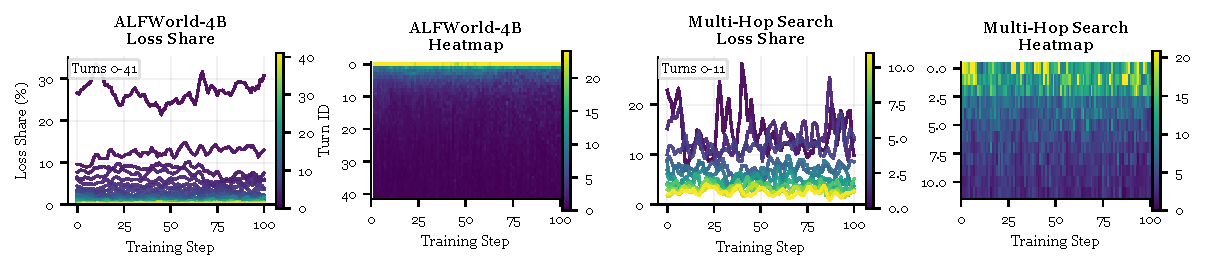
\includegraphics[width=\textwidth]{figures/fig_loss_share_turn_lines_alfworld4b_multihop_baseline.pdf}
  \caption[Turn-level KL loss-share under trajectory-level aggregation]{Turn-level KL loss-share under the vanilla trajectory-level KL objective. Line panels show one smoothed training-step curve per reliably observed turn; heatmaps show the raw step-by-turn loss-share values. The metric is the fraction of the current batch's raw KL loss mass contributed by turn $t$.}
  \label{fig:diag-loss-share}
\end{figure*}

Figure~\ref{fig:diag-loss-share} shows that the KL loss is mainly concentrated in the early turns. In ALFWorld-4B, turn~0 alone uses about a quarter of the KL budget. The first three turns take nearly half. The reliable deep third receives only $3.6$--$4.5\%$ of the KL loss. In Multi-Hop Search, the effect is weaker, but the first three turns still take $38$--$40\%$ of the budget. The reliable deep third gets only $11$--$13\%$. This makes sense: not every rollout reaches the deep turns, so there are fewer tokens from deep turns in a batch. The KL loss in shallow turns is also larger. As a result, the KL loss is mostly assigned to earlier turns. The observations lead to two main conclusions:

\textbf{(1) Trajectory-level normalization creates a budget mismatch.}
This is not a claim that every deep turn is more valuable. The point is simpler:
the trajectory-level reducer spends loss by token mass and realized KL mass. It
can therefore keep most updates near the shallow prefix even when later turns
still contain correction signal. Table~\ref{tab:diag-loss-aggregation} quantifies
this with the same runs and the same reliable prefixes as
Figure~\ref{fig:diag-loss-share}.

\textbf{(2) A hard turn-level replacement may also be too crude.}
The other extreme gives each observed turn the same total weight. This removes
the shallow token-count bias, but it may also ignore reliability. In ALFWorld-4B,
the reliable deep third has only $31$--$42\%$ of the shallow prefix's raw KL. In
Multi-Hop Search, the deep third has comparable raw KL, but only about
$16$--$17\%$ survivor support. Equalizing all turns from the beginning would
therefore amplify weaker or lower-support estimates too early.

\begin{table*}[tbp]
  \centering
  \caption[Loss-allocation diagnostics]{Loss-allocation diagnostics from vanilla OPD baselines.
  Deep/shallow ratios compare the deepest third of the reliable turn prefix with
  the shallowest third, using the same prefixes as
  Figure~\ref{fig:diag-loss-share}. Raw KL is the actual optimization signal.
  ``Deep support'' is survivor coverage in the deepest third, and ``Deep loss
  budget'' is the fraction of total raw-KL loss mass assigned to that deepest
  third by the trajectory-level objective.}
  \label{tab:diag-loss-aggregation}
  \small
  \setlength{\tabcolsep}{6pt}
  \begin{tabular}{@{}>{\raggedright\arraybackslash}m{3cm}>{\centering\arraybackslash}m{1.4cm}>{\centering\arraybackslash}m{2.3cm}>{\centering\arraybackslash}m{2.2cm}>{\centering\arraybackslash}m{2.2cm}@{}}
  \toprule
  Task & Phase & \shortstack{Deep/Shallow\\raw KL} & \shortstack{Deep\\support} & \shortstack{Deep loss\\budget} \\
  \midrule
  ALFWorld & early & 31\% & 23.0\% & 3.6\% \\
  ALFWorld & late & 42\% & 18.2\% & 4.5\% \\
  Multi-Hop Search & early & 90\% & 17.3\% & 12.9\% \\
  Multi-Hop Search & late & 92\% & 15.5\% & 11.1\% \\
  \bottomrule
  \end{tabular}
\end{table*}
\FloatBarrier
  

% \begin{table}[htbp]
% \centering
% \caption[Loss-allocation diagnostics]{Loss-allocation diagnostics from vanilla OPD baselines.
% Deep/shallow ratios compare the deepest third of observed turns with the
% shallowest third. Raw KL is the actual optimization signal; $\NKL$ is an
% entropy-normalized local correction diagnostic. ``Deep support'' is survivor
% coverage in the deepest third, and ``Deep loss budget'' is the fraction of total
% raw-KL loss mass assigned to that deepest third by the trajectory-level
% objective.}
% \label{tab:diag-loss-aggregation}
% \small
% \begin{tabular}{@{}llcccc@{}}
% \toprule
% Task & Phase & \shortstack{Deep/Shallow\\raw KL} & \shortstack{Deep/Shallow\\local corr. ($\NKL$)} & \shortstack{Deep\\support} & \shortstack{Deep loss\\budget} \\
% \midrule
% ALFWorld & early & 0.05 & 0.62 & 9.6\% & 0.3\% \\
% ALFWorld & late & 0.17 & 0.61 & 7.1\% & 1.5\% \\
% Multi-hop search & early & 0.72 & 0.83 & 1.7\% & 5.5\% \\
% Multi-hop search & late & 0.73 & 0.70 & 1.6\% & 3.7\% \\
% \bottomrule
% \end{tabular}
% \end{table}

\subsection{Summary: Two Budget Mismatches}
\label{sec:diag:fail}

The diagnosis isolates two budget mismatches in vanilla agent OPD:

\textbf{First, an external mismatch.} Rollout depth is fixed, but the
survivor-weighted local correction signal and the survivor population both vary
sharply with turn depth. Collecting to the maximum horizon can spend rollout
compute on turns whose observable correction mass is low or whose estimates are
dominated by a small survivor subset. This motivates an adaptive rollout-depth
controller that decides \textbf{how far to collect}.

\textbf{Second, an internal mismatch.} After a trajectory is collected,
trajectory-level normalization starts from uniform token weighting and realizes a
shallow KL-mass concentration. 
However, in agent tasks, turns with few tokens are not necessarily less important. After mastering initial interactions, remaining errors are often in deeper decision turns, yet the token-weighted objective assigns little loss budget to these steps.
This motivates a progressive turn-level weighting
controller that decides \textbf{where the collected loss mass should go}.

These two failures have the same underlying structure: the useful unit of
supervision in a long-horizon agent is not a flat token position, but a
turn-conditioned decision embedded in an evolving interaction trace.

% \begin{proposition}[Depth proxy for rollout control]
% \label{prop:depth-proxy}
% Let $\tau_{\mathrm{done}}$ be the first depth at which the success-completion
% CDF reaches full coverage, used as an empirical proxy for the task's
% dependency-closure depth, and let $H_{\mathrm{ctrl}}$ be the online rollout-depth
% proxy constructed in Section~\ref{sec:method:A}. The useful collection depth is
% controlled by
% \begin{equation}
% H_{\mathrm{ctrl}}=\max(\Heff,\Hcov).
% \end{equation}
% In the simple regime where tool dependencies are shallow or independent,
% $\tau_{\mathrm{done}}$ collapses to a shallow turn and the useful-depth problem
% reduces to the raw-KL signal centroid; in long-horizon tasks, the success-coverage
% floor prevents the efficiency side from truncating still-needed dependency chains.
% \end{proposition}

% This proposition bridges the diagnosis to adaptive rollout depth: the method
% should not use a fixed rollout horizon, but should track both the
% survivor-weighted raw-KL centroid and the task-coverage boundary.
